\documentclass[11pt]{article}
\usepackage[spanish]{babel}
\usepackage{graphicx}
\graphicspath{ {./imagenes/} }

\title{Proyecto \#2: Programación paralela\\
Algoritmo de Dijkstra\\
\large Estructura de datos y algoritmos II}

\author{Cabello, Sofía
\and López, Ricardo
\and Núñez, Diego}

\begin{document}

\maketitle{}

\section{Algoritmo utilizado y su implementación }


Primero que nada, es importante aclarar que nos basamos en código encontrado en (Matloff, 2012) con algunas modificaciones, ya que se generaba una condición de carrera que será explicada más adelante.
\par 
¿Cómo correr el programa? El programa recibe dos parámetros desde la terminal, uno para indicar el número de nodos que tendrá el grafo aleatorio (llamado nv dentro del programa) y otro para indicar si se deben imprimir los resultados. Aunque esta última opción parece un poco extra o tonta, fue muy útil para las pruebas de rendimiento.
\par 
El programa comienza llenando la matriz de adyacencia del grafo. Como el programa crea grafos ponderados bidireccionales, no se ingresan valores negativos a la matriz. Primero se llena una mitad y después los valores son copiados a la otra, ya que la matriz debe ser simétrica.
\par 
Después, se inicializan los valores de un arreglo de nv espacios que indica si un nodo todavía no ha sido visitado. Al nodo 0 le corresponde el espacio 0 de este arreglo, al 1 el espacio 1 y así sucesivamente hasta nv-1. Cuando existe un valor de 1, entonces el nodo todavía no ha sido visitado. A este arreglo se le conoce como no notDone.
\par
Junto al arreglo anterior se inicializan los valores de otro arreglo llamado mind, que almacena las distancias mínimas almacenadas hasta el momento hacia cada nodo. Por defecto, estas distancias se inicializan con el valor de la arista que conecta directamente a cualquier nodo con el nodo 0. Además, este arreglo almacena datos de tipo usigned, ya que esta versión del algoritmo que no utiliza una cola de prioridad no funciona con pesos negativos. 
\par
Teniendo todo listo comienza el algoritmo en sí. Se encuentra el constructor parallel, lo que significa que a partir de este punto se utilizarán varios hilos. Primero, se inicializan tres variables, step, mymv y mymd. La primera variable indica que nodo se está revisando en un momento. Cada nodo es revisado una vez, por esta razón step va desde 0 hasta nv-1. La segunda y la tercera sirven para almacenar de manera local para los hilos cual es el nodo más cercano al nodo inicial que han encontrado de manera individual. 
\par
Después, en un bloque single, se inicializa los valores de mv y md. Estas variables almacenan el nodo más cercano al nodo inicial de entre todos los encontrados por todos los hilos. La variable md se inicializa en -1 (Que, como las distancias son de tipo unsigned, en realidad representa el mayor entero posible) y mv en 0. Esto es así ya que la distancia mínima encontrar al inicio del algoritmo es presuntamente infinita y el vértice hacia el que hay esa distancia es presuntamente inexistente hasta que se indique lo contrario.
\par
Después, en una estructura omp for, cada hilo trabaja con un subconjunto de los nodos adyacentes al nodo 0, cada uno determina cual es el más cercano de su subconjunto. Luego, en una estructura critical, cada hilo pasa uno por uno a revisar si su menor valor encontrado es menor al ya existente. Si es así, se actualizan mv y md para referir al nodo más cercano en la iteración.
\par
En una estructura single, se marca a este nuevo nodo más cercano como revisado, así que en la siguiente iteración ya no podrá ser seleccionado como el nodo más cercano al inicial.
\par
Finalmente, en un ciclo for también paralelizado, se calculan distancias hacia todos los demás nodos y si es menor a la distancia más corta ya existente, se actualiza. 
\par
En este punto es donde se generaba la condición de carrera. OpenMP no asegura la manera ni el orden en cómo se ejecutarán las iteraciones de una estructura for. Por esta razón, un hilo podía terminar su parte primero y llegar a esta sección antes de que el otro, actualizando las distancias antes de que los demás hilos propusieran un nodo para ser el más pequeño en general. Para arreglar esto, se agregó una barrera después del critical, de esta manera se espera que todos los hilos actualicen mv y md si lo requieren antes de continuar. 
\par
En la siguiente iteración se repite el proceso, solo que esta vez ya estará marcado el nodo más cercano que se utilizó en la iteración anterior, por lo que ahora se ocupará el segundo más cercano y así sucesivamente hasta que no haya más nodos adyacentes al nodo inicial.


\begin{figure}[!htbp]
\centering
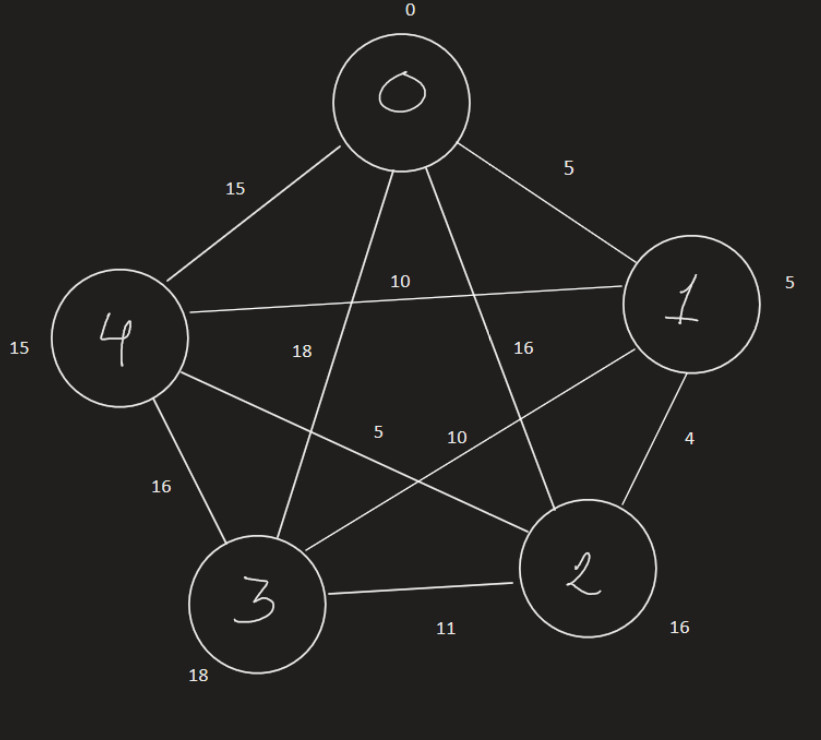
\includegraphics[scale = .5]{grafos1}
\caption{Grafo inicial}
\end{figure}

\begin{figure}[!htbp]
\centering
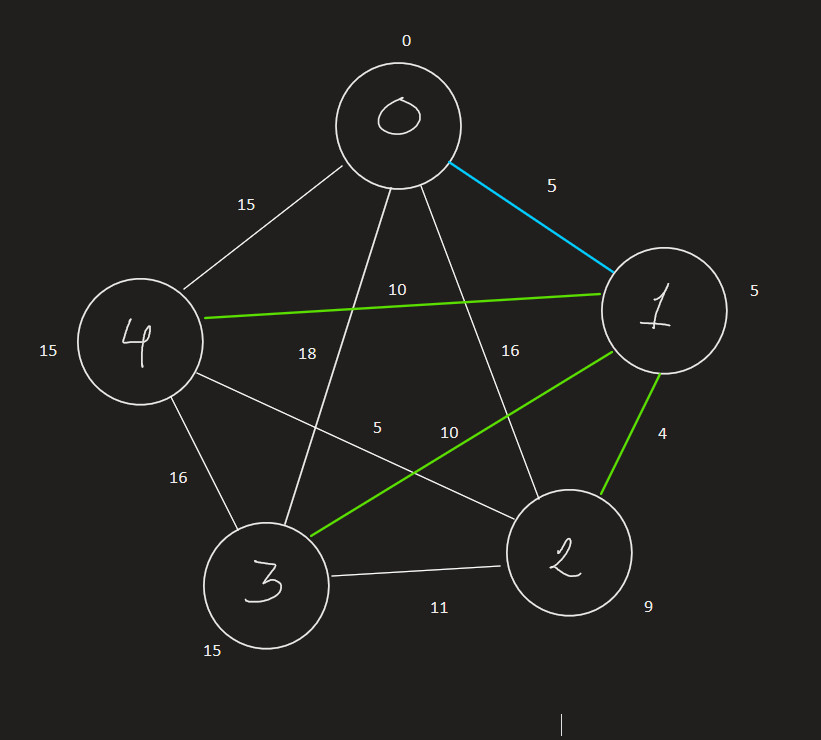
\includegraphics[scale = .5]{grafos2}
\caption{Primero se visita al nodo al nodo adyacente más cercano al origen.}
\end{figure}


\begin{figure}[!htbp]
\centering
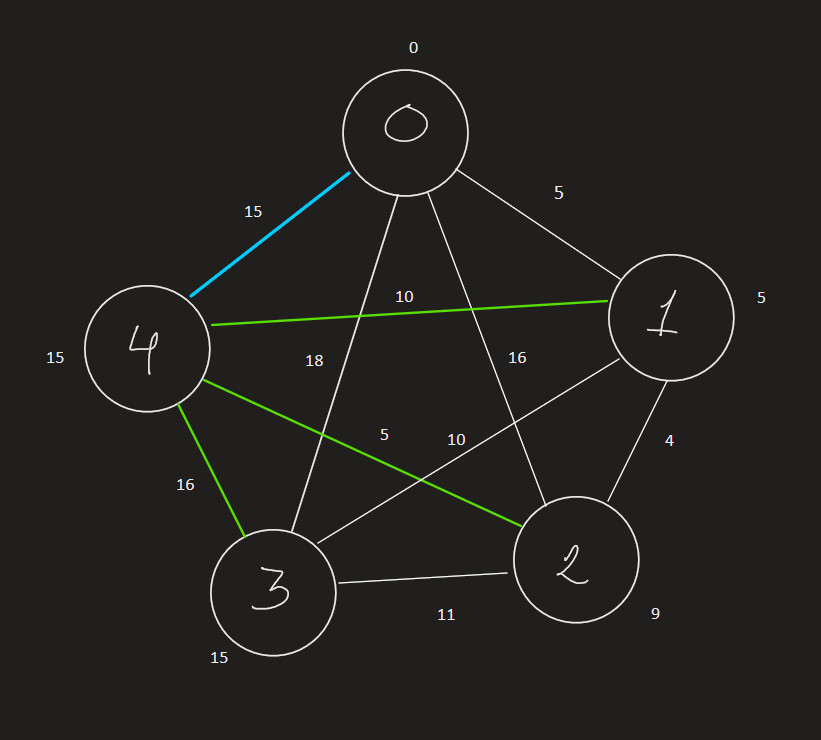
\includegraphics[scale = .5]{grafos3}
\caption{Después se visita el segundo más cerca.}
\end{figure}

\begin{figure}[!htbp]
\centering
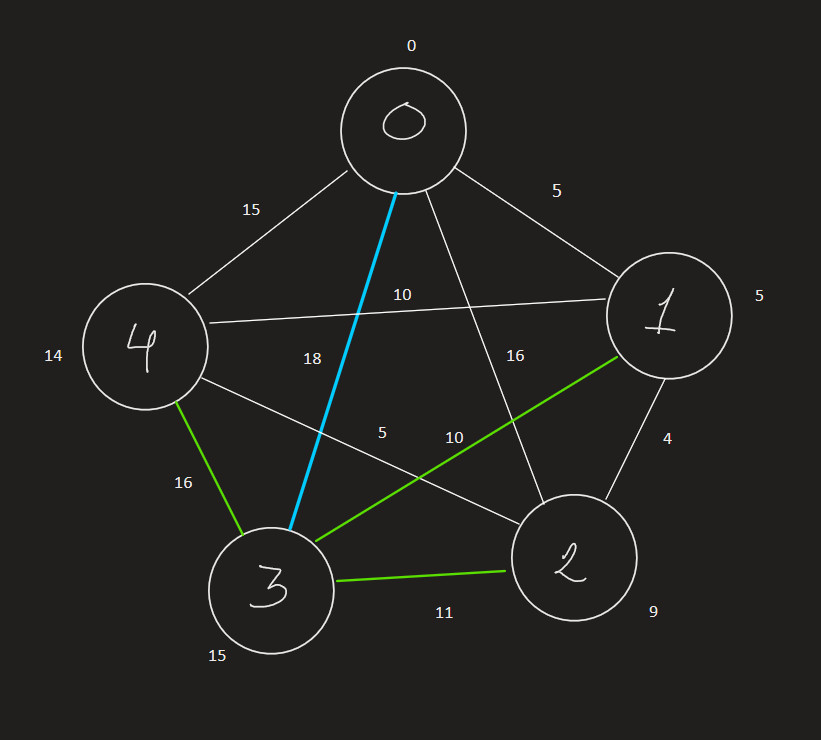
\includegraphics[scale = .5]{grafos5}
\caption{El algoritmo finaliza una vez que se visitó el más lejano.}
\end{figure}
\end{document}
